\newcount\mycount
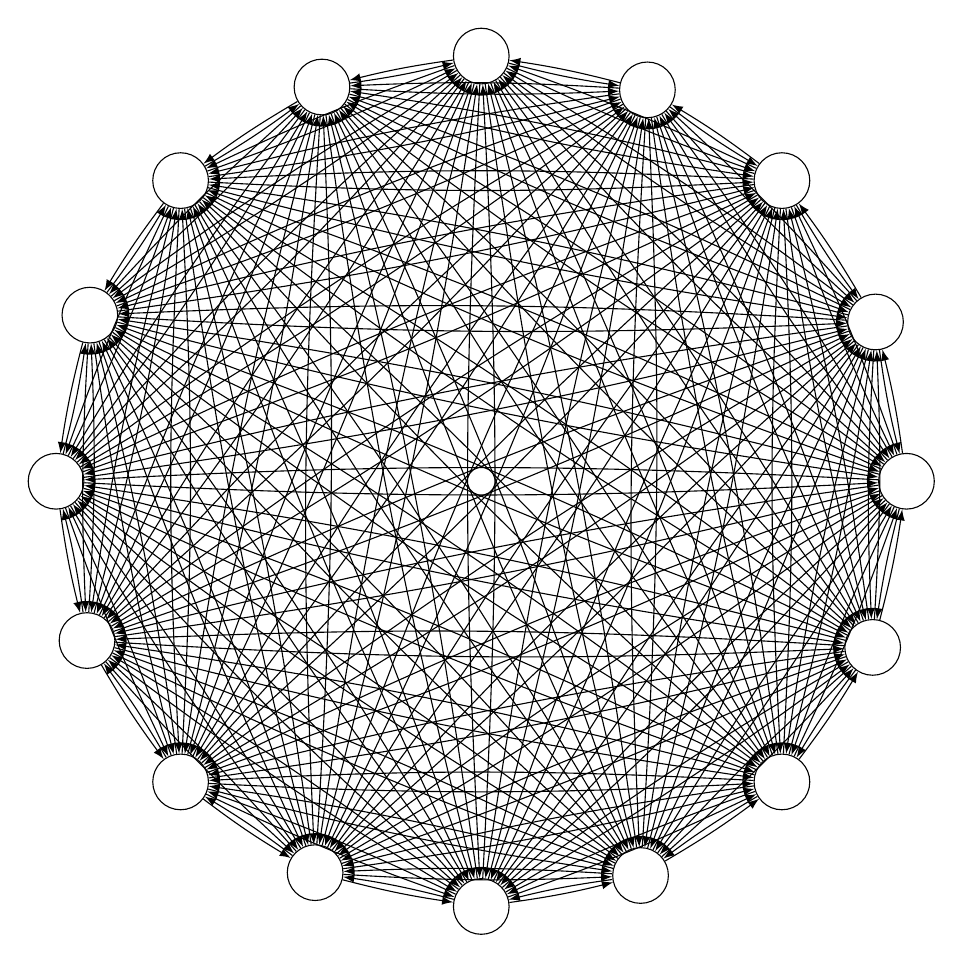
\begin{tikzpicture}[transform shape]
  %the multiplication with floats is not possible. Thus I split the loop in two.
  \foreach \number in {1, ..., 8}{
    % Computer angle:
    \mycount=\number
    \advance\mycount by -1
    \multiply\mycount by 45
    \advance\mycount by 0
    \node[draw, circle, inner sep=0.25cm] (N-\number) at (\the\mycount:5.4cm) {};
  }
  \foreach \number in {9, ..., 16}{
    % Computer angle:
    \mycount=\number
    \advance\mycount by -1
    \multiply\mycount by 45
    \advance\mycount by 22.5
    \node[draw, circle, inner sep=0.25cm] (N-\number) at (\the\mycount:5.4cm) {};
  }
  \foreach \number in {1, ..., 15} {
    \mycount=\number
    \advance\mycount by 1
    \foreach \numbera in {\the\mycount, ..., 16} {
      \path (N-\number) {
        edge[-latex, bend right=3] (N-\numbera)
        edge[latex-, bend left=3] (N-\numbera)
      };
    }
  }
\end{tikzpicture}
